\documentclass[10pt,letterpaper]{article}
\usepackage{multirow}
\usepackage{hyperref}
\usepackage{cogsci}
\usepackage{pslatex}
\usepackage{amsmath}
\usepackage{amsfonts}
\usepackage{setspace}
\usepackage{apacite}
\usepackage{graphicx}
\usepackage{caption}
\usepackage{subcaption}
\usepackage{etex}
\usepackage{color}
\usepackage[usenames,dvipsnames,svgnames,table]{xcolor}
\usepackage[usenames,dvipsnames]{xcolor}
\usepackage{tikz}
\usepackage{array}

%\usepackage{todonotes}
 \newcommand{\xivpt}{\fontsize{15pt}{15pt}}
\usetikzlibrary{decorations.shapes}
\title{\scalebox{0.9}{The Funny Thing About Incongruity: A Computational Model of Humor in Puns}}
 
 \author{{\large {\bf Justine T. Kao$^1$} (justinek@stanford.edu)}, {\large {\bf Roger Levy$^2$} (rlevy@ucsd.edu)}, {\large {\bf Noah D.~Goodman$^1$} (ngoodman@stanford.edu)}\\
  $^1$Department of Psychology, Stanford University. $^2$Department of Linguistics, UC San Diego. }
 
 

\begin{document}

\maketitle

\begin{abstract}
\emph{Researchers showed the robot ten puns, hoping that one of them would make it laugh. Unfortunately, no pun in ten did.}\\

What makes something funny? Humor theorists posit that incongruity---perceiving a situation from different viewpoints and finding the resulting interpretations to be incompatible---contributes to sensations of mirth. In this paper, we use a computational model of sentence comprehension to formalize incongruity and test its relationship to humor in puns. By combining a noisy channel model of language comprehension and standard information theoretic measures, we derive two dimensions of incongruity---ambiguity of meaning and support of different viewpoints---and use them to predict humans' judgments of funniness. Results showed that both ambiguity and support are significant predictors of humor. Additionally, our model automatically identifies specific features of a pun that make it amusing. We thus show how a probabilistic model of sentence comprehension can help explain essential features of the complex phenomenon of linguistic humor.

\textbf{Keywords:} 
Humor; language understanding; probabilistic models
\end{abstract}
\section{Introduction}

\subsection{Motivate humor and its importance}
\begin{itemize}
\item[(1)] Humor is everywhere! It has cognitive, social, and health implications.
\end{itemize}
\subsection{Humor theories: incongruity and resolution}
\begin{itemize}
\item[(1)] Introduce existing theories of humor
\item[(2)] Frame incongruity as presence of two equally likely interpretations
\item[(3)] Frame resolution as supporting context for each interpretation
\item[(4)] Introduce noisy channel and relevance (do this here or after introducing puns?)
\end{itemize}
\subsection{Puns as case study}
\begin{itemize}
\item[(1)] Why language/meaning is hard
\item[(2)] Why puns are relatively simpler
\item[(3)] Walk through an example pun

\end{itemize}

\section{Model}
\begin{itemize}
\item[(1)] Introduce language model (gist + ngram), plot generative model
\item[(2)] Introduce formal measures of ambiguity and support
\end{itemize}

\begin{figure}
\centering
\tikzset{decorate sep/.style 2 args=
{decorate,decoration={shape backgrounds,shape=circle,shape size=#1,shape sep=#2}}}
\begin{tikzpicture}
\tikzstyle{place}=[circle,draw,inner sep=2pt,minimum size=0.95cm]
 \tikzstyle{plate}=[rectangle,draw,inner sep=0pt]
 \node[place] (m) at (0,3) {$m$};
 \node[place] (w1) at (-2,1.5) {$w_1$};
 \node[place] (w2) at (-1,1.5) {$w_2$};
 \node[place] (h) at (0.5,1.5) {$h$}; 
 \node[place] (wn) at (2,1.5) {$w_n$};
 \node[place] (f1) at (-2, 0) {$f_1$};
 \node[place] (f2) at (-1, 0) {$f_2$};
\node[place] (fh) at (0.5, 0) {$f_h$};
\node[place] (fn) at (2, 0) {$f_n$};
 %\node[place] (wordsprior) at (0,4.5) {$\wordsprior$};
\draw [->] (m) -- (w1);
\draw [->] (m) -- (w2);
\draw [->] (m) -- (h);
\draw [->] (m) -- (wn);
\draw [->] (f1) -- (w1);
\draw [->] (f2) -- (w2);
\draw [->] (fh) -- (h);
\draw [->] (fn) -- (wn);
\draw[decorate sep={0.3mm}{1.65mm},fill] (-0.41,1) -- (-0.05,1);
\draw[decorate sep={0.3mm}{1.65mm},fill] (-0.41,-0.5) -- (-0.05,-0.5);
\draw[decorate sep={0.3mm}{1.65mm},fill] (1.09,1) -- (1.45,1);
\draw[decorate sep={0.3mm}{1.65mm},fill] (1.09,-0.5) -- (1.45,-0.5);
\end{tikzpicture}
\caption{Generative model of a sentence. Each word $w_i$ is generated based on the sentence topic $m$ if the indicator variable $f_i$ puts it in semantic focus; otherwise it is generated as noise (from a trigram distribution). }
\label{generativeModel}
\end{figure}
\begin{align}
P(m, \vec f | \vec w) = P(m | \vec w) P(\vec f | m, \vec w) 
\end{align}

\subsection{Measures}
\subsubsection{Ambiguity} \begin{align}
P(m | \vec w) &= \sum_{\vec f} P(m, \vec f | \vec w) \\
&\propto \sum_{\vec f} P(\vec w | m, \vec f) P(m) P(\vec f) \\
&= \sum_{\vec f} \bigg (P(m)P(\vec f)\prod_i P(w_i | m, f_i) \bigg)
\end{align}
%From Bayes' theorem, this is proportional to the following:
%$$
%\sum_{\vec f} P(\vec w | m, \vec f) P(m) P(\vec f)= \sum_{\vec f} \bigg (P(m)P(\vec f)\prod_i P(w_i | m, f_i) \bigg)
%$$
\[
    P(w_i | m, f_i) = 
\begin{cases}
    P(w_i),& \text{if } f=0\\
    P(w_i | m), &\text{if } f=1\\
\end{cases}
\]
\subsubsection{Support}
Under construction... 
\begin{align}
P(\vec f | m, \vec w) \propto P(\vec w | m, \vec f) P(\vec f | m)
\end{align}

 %Once we derive $P(\vec f | m_1, \vec w)$ and $P(\vec f | m_2, \vec w)$, we compute its symmetrised KL divergence as a measure of distinctiveness.
\subsection{Model of meaning}
\begin{itemize}
\item[(1)] Describe relatedness ratings as approximation of PMI
$$
R(w, m)= {\log \frac{P(w, m)}{P(w)P(m)}} = \log \frac{P(w | m)}{P(w)} = \log P(w | m) - \log P(w)
$$
\item[(2)] Describe empirically driven model of meaning
\begin{align}
P(w | m) = e^{R'(w, m) + z} P(w)
\end{align}
\end{itemize}

\section{Evaluation}
\subsection{Experiment 1: Identical Homophone Puns}
\begin{itemize}
\item[(1)] Describe identical homophone corpus (should we include de-punned?)
\item[(2)] Describe experiment to obtain relatedness ratings
\item[(3)] Describe experiment to obtain funniness ratings
\item[(4)] Show some plots summarizing data
\item[(5)] Regression model using ambiguity and support to predict funniness
\item[(6)] Plots summarizing results
\end{itemize}


\begin{figure*}[t]
\mbox{
\begin{subfigure}{0.45\textwidth}
\scalebox{0.38}{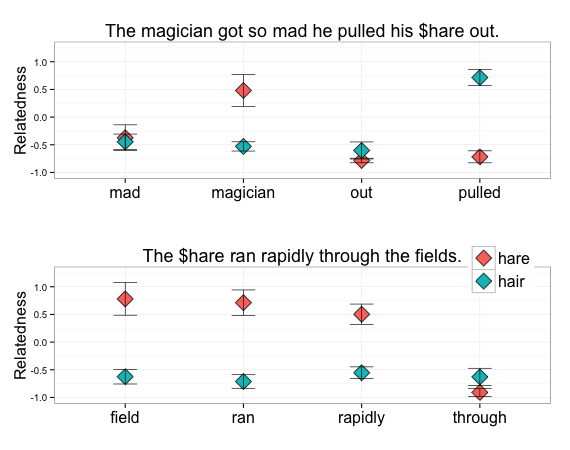
\includegraphics{Plots/relatedness_example.png}}
\subcaption{Relatedness of each word with candidate meanings}
\end{subfigure}
\begin{subfigure}{0.29\textwidth}
\scalebox{0.4}{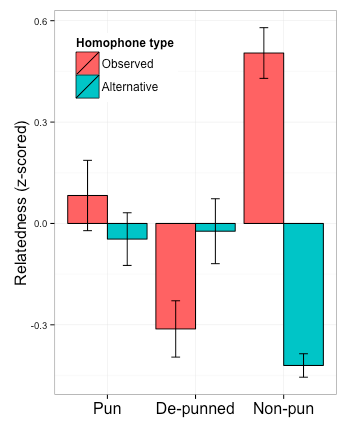
\includegraphics{Plots/ave_relatedness.png}}
\subcaption{Average relatedness }
\end{subfigure}
\begin{subfigure}{0.31\textwidth}
\scalebox{0.4}{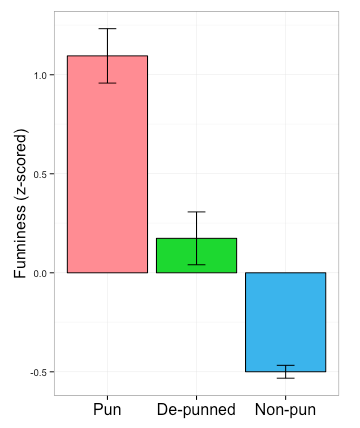
\includegraphics{Plots/ave_funniness.png}}
\subcaption{Average funniness ratings}
\end{subfigure}
}
\caption{(a) In the example pun (top), two candidate meanings of $h$ are each more related to a subset of the content words. In the non-pun, only one candidate meaning is more related. (b) Content words are similarly related to both candidate meanings in puns; more related to alternative meanings in de-puns; more related to observed meanings in non-pun. (c) Funniness varies across the sentence types in a pattern that reflects the balance of relatedness to candidate meanings shown in (b).}
\label{ratings_analyses}
\end{figure*}

\begin{figure}[t]
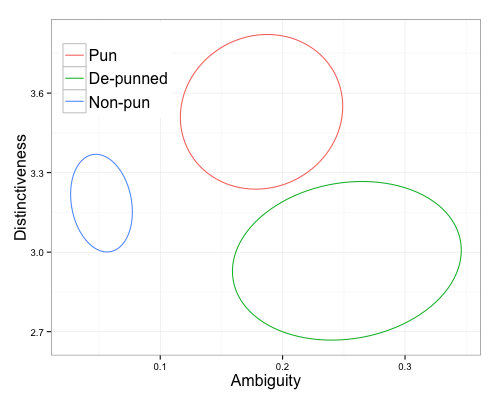
\includegraphics[width=80mm, height=60mm] {Plots/ellipse_camera.png}
\caption{Standard error ellipses of ambiguity and distinctiveness across sentence types. Puns score higher on ambiguity and distinctiveness; de-puns are less supported by distinct focus sets; non-puns have low ambiguity.}
\label{ellipse}
\end{figure}

\begin{figure}[t]
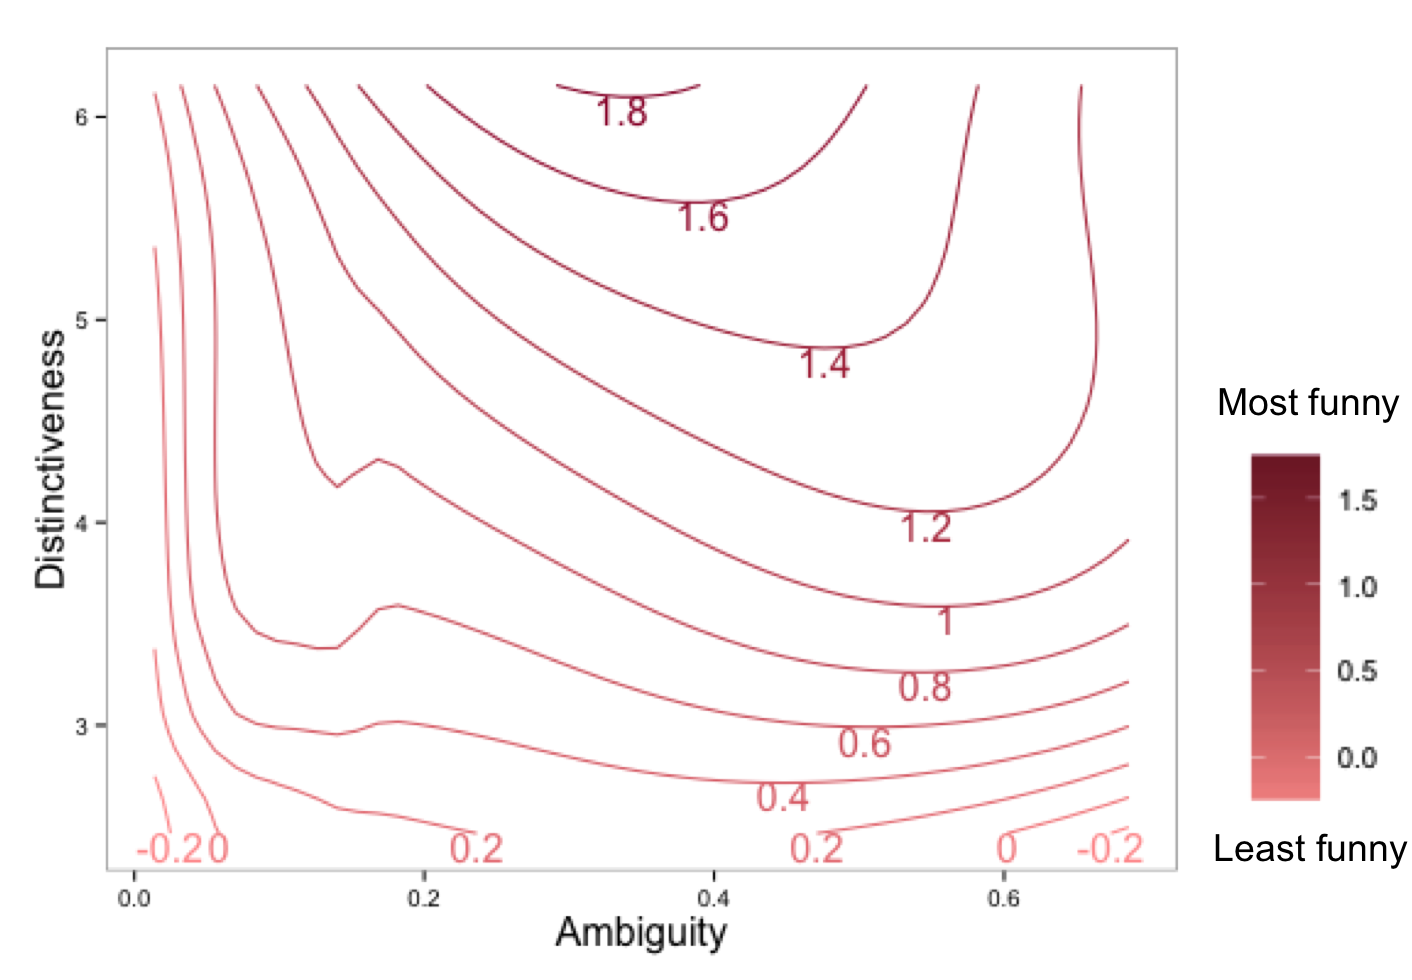
\includegraphics[width=90mm, height=60mm]{Plots/contour_camera_marked.png}
\caption{Funniness contours smoothed using a 2-D Loess regression with ambiguity and disjointedness measures as predictors. Sentences become funnier as they move to high ambiguity and distinctiveness space.}
\label{contour}
\end{figure}
\subsection{Experiment 2: Near Homophone Puns}

\begin{itemize}

\begin{figure}[t]
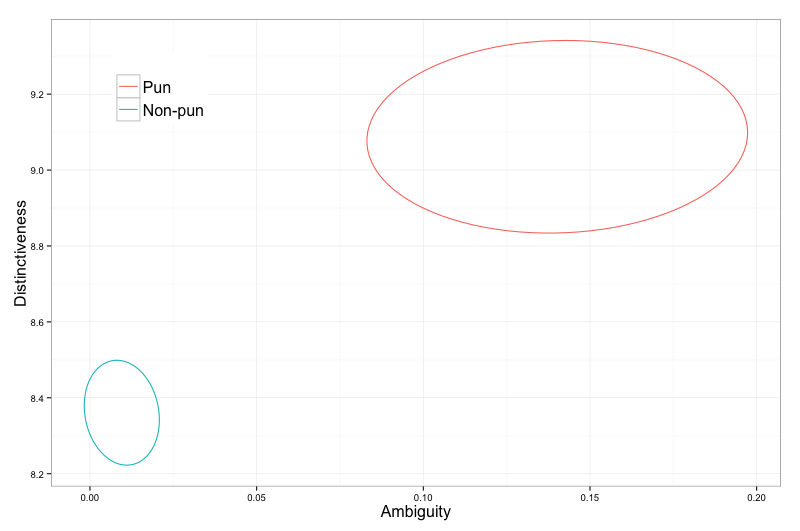
\includegraphics[width=80mm, height=60mm] {Plots/ellipse.png}
%\end{figure}

%\begin{figure}[t]
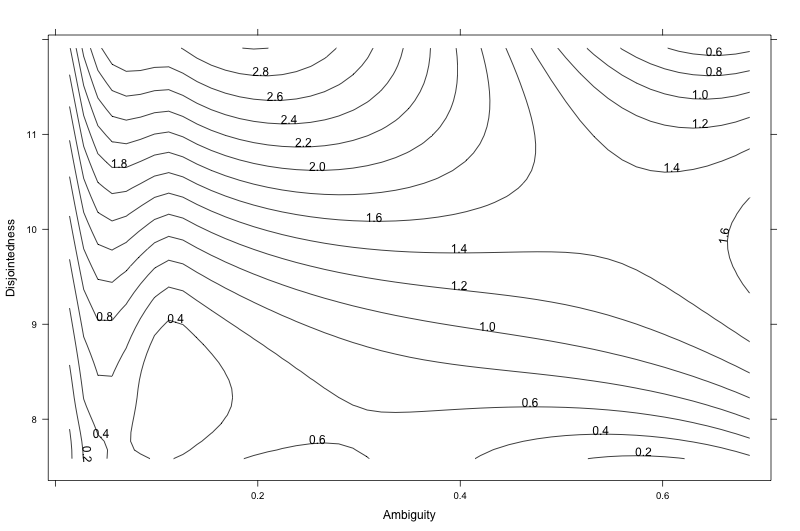
\includegraphics[width=80mm, height=60mm]{Plots/contour.png}
\end{figure}

\item[(1)] Motivate purpose of examining near homophone puns: more fine-grained. Phonetic distance may introduce more or less noise that affects the delicate balance of ambiguity and support
\item[(2)] Describe near homophone corpus
\item[(3)] Describe experiment to obtain relatedness ratings
\item[(4)] Describe experiment to obtain funniness ratings
\item[(5)] Show some plots summarizing data
\item[(6)] Regression model using ambiguity and support to predict funniness, without accounting for phonetic distance
\item[(7)] Regression model using ambiguity and support to predict funniness, adding phonetic distance (hopefully will get better results)
\item[(8)] Table showing focus sets
\end{itemize}



\section{Discussion}

\begin{itemize}
\item[(1)] Both experiments and their comparison suggest that funny puns exploit a delicate balance of meanings. By building a model of meanings and formally measuring that balance, we can predict funniness quite well.
\item[(2)] A relatively simple model of language and meaning can shed light on complex phenomena
\end{itemize}



\bibliographystyle{apacite}

\setlength{\bibleftmargin}{.125in}
\setlength{\bibindent}{-\bibleftmargin}

%\bibliography{pun_bib}


\end{document}

